\documentclass[a4paper,10pt]{article}
\usepackage[utf8]{inputenc}
\newcommand{\myparagraph}[1]{\paragraph{#1}\mbox{}\\}
\usepackage[a4paper,margin=3.5cm]{geometry} %Sets the page geometry
\usepackage{url}
\usepackage{dirtytalk}
\usepackage{graphicx} % Package for \includegraphics
\usepackage{wrapfig} % Figure wrapping
\usepackage[T1]{fontenc} % Output font encoding for international characters
\setlength{\parskip}{1em} % Set space when paragraphs are used
\usepackage{amssymb}
\usepackage{amsmath}
\usepackage{tcolorbox}
\usepackage{mathtools}

\usepackage{standalone}
\usepackage{tikz}
\usetikzlibrary{decorations.pathmorphing,patterns,arrows.meta,calc}

% Lets you use \blankpage to make a blank page
\newcommand{\blankpage}{
\newpage
\thispagestyle{empty}
\mbox{}
\newpage
}

\newcommand{\R}{\mathbb{R}}
\newcommand{\fnet}{F^{\text{net}}}
\newcommand{\bx}{\mathbf{x}}
\newcommand{\bfnet}{\mathbf{\fnet}}
\newcommand{\ddbx}{\ddot{\bx}}
\newcommand{\ddx}{\ddot{x}}
\newcommand{\kN}{\text{kN}}

\title{Numerical Method of hlsimII}
\author{Asger Limkilde}


% Other
\DeclarePairedDelimiter\floor{\lfloor}{\rfloor} %Floor function

\begin{document}

\maketitle

This document describes the numerical method used in the highline simulator. It's is described from an math/numerics point of view. For implementation details not covered here, look in the source code.


\tableofcontents

\section{Introduction}
\label{sec:intro}
My goal with this simulator was to gain a better understanding of the forces involved in highline leash- and backup-falls. 

A very useful simulation tool exists already [CITE ISA Backupfall simulator]. However this simulator had some short comings that I wanted to address. Namely, it assumes that the total mass of the system is located at the position of the slackliner. This makes the simulator increasingly inaccurate when lines become longer and heavier. Additionally it would not take into account that in a leash fall, the line flicks up quickly, and some of the energy of the falling slackliner is dissipated through the wave propagation down the line.

So in this work, I was curious to see what would happen if I did a full simulation of the dynamics involved in highline falls. So where [CITE] relied on a simple calculation using energy conservation, in this work I try to do a full time-integration of the highline system when a fall occurs.

This document is structured as follows; In Section~\ref{sec:nummethod} I will introduce the numerical model used in this work. In Section~\ref{sec:impl} I will give a few pointers on how it was implemented, and a few comments on the things that didn't work too well. In Section~\ref{sec:compare_ISA} I will discuss how this method differ from the \texttt{ISA backupfall simulator} [CITE] by Augustin~Moinat, and look at how the result differ for some examples. Finally in Section~\ref{sec:concl} I conclude and discuss some future work that could be interesting.

A seperate document will include a validation by comparing in more detail to \texttt{ISA backupfall simulator} [CITE] and to real life experiments also by A. Moinat et al.

\section{The Numerical Method}
\label{sec:nummethod}

\subsection{Base model of a highline}%
\label{sec:basemodel}

The approach we take to model the highline system, is that we imagine that the webbing consists of a chain of springs, with point masses in between. The setup is illustrated in Figure~\ref{fig:spring-chain}.  
%
  \begin{figure}[htbp]
    \centering
    % Lumped mass model of the webbing: overview of the chain and a zoom on node i.
% Build:  pdflatex spring_chain.tex && pdftops -eps spring_chain.pdf spring_chain.eps
\documentclass[tikz,border=4pt]{standalone}
\usetikzlibrary{decorations.pathmorphing,patterns,arrows.meta,calc}

\begin{document}
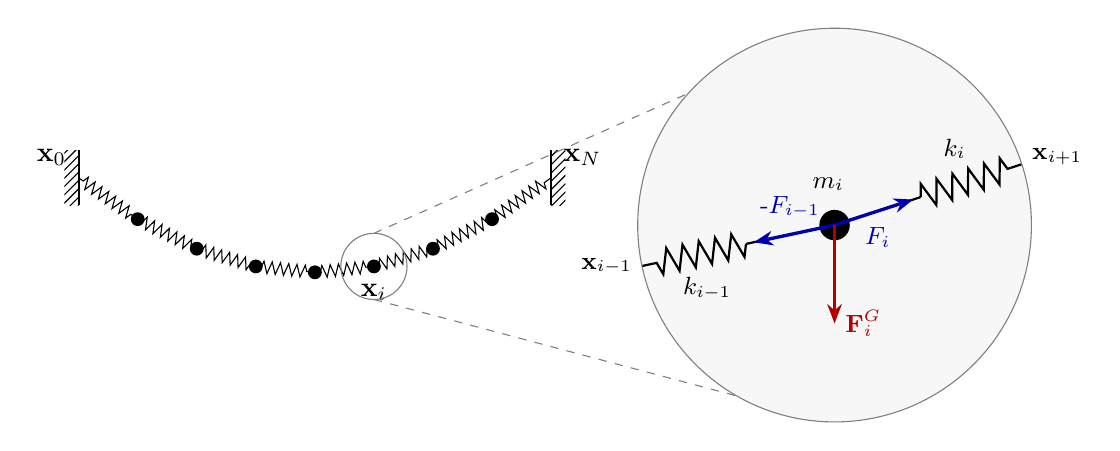
\begin{tikzpicture}[
    mass/.style={circle,fill=black,inner sep=0pt,minimum size=5pt},
    bigmass/.style={circle,fill=black,inner sep=0pt,minimum size=11pt},
    spring/.style={decorate,decoration={zigzag,segment length=3pt,amplitude=2.2pt,
                   pre length=2pt,post length=2pt}},
    bigspring/.style={decorate,decoration={zigzag,segment length=6pt,amplitude=4.5pt}},
    force/.style={-{Stealth[length=7pt]},very thick},
    zoomline/.style={gray,dashed,thin},
  ]

  % ---------------------------------------------------------------- overview
  % Parabolic sag, y = -s (1 - ((x - 3)/3)^2), N = 8 edges
  \def\s{1.2}
  \foreach \j in {0,...,8} {
    \pgfmathsetmacro{\x}{0.75*\j}
    \pgfmathsetmacro{\y}{-\s*(1-((\x-3)/3)^2)}
    \coordinate (n\j) at (\x,\y);
  }
  \foreach \j [evaluate=\j as \jn using int(\j+1)] in {0,...,7}
    \draw[spring] (n\j) -- (n\jn);
  \foreach \j in {1,...,7} \node[mass] at (n\j) {};

  % Fixed anchors
  \foreach \a/\d in {n0/-1, n8/1} {
    \fill[pattern=north east lines] ($(\a)+(0,-0.35)$) rectangle ($(\a)+(0.18*\d,0.35)$);
    \draw[thick] ($(\a)+(0,-0.35)$) -- ($(\a)+(0,0.35)$);
  }
  \node[above left=1pt]  at (n0) {$\mathbf{x}_0$};
  \node[above right=1pt] at (n8) {$\mathbf{x}_N$};
  \node[below=3pt]       at (n5) {$\mathbf{x}_i$};

  % ---------------------------------------------------------------- zoom
  \def\r{0.42}   % radius of the small circle
  \def\R{2.5}    % radius of the zoom panel
  \coordinate (Z) at (9.6,-0.6);
  \draw[gray] (n5) circle (\r);
  \draw[zoomline] ($(n5)+(0,\r)$)  -- ($(Z)+(0,\R)$);
  \draw[zoomline] ($(n5)+(0,-\r)$) -- ($(Z)+(0,-\R)$);

  \begin{scope}
    \clip (Z) circle (\R);
    \fill[gray!6] (Z) circle (\R);

    % One edge: a lead, then a spring, then a lead.
    % #1 = angle of the edge, #2 = label of its spring
    \newcommand{\kedge}[2]{
      \begin{scope}[shift={(Z)},rotate=#1]
        \draw[thick] (0,0) -- (1.15,0);
        \draw[thick,bigspring] (1.15,0) -- (2.35,0);
        \draw[thick] (2.35,0) -- (3.2,0);
        \node[font=\small] at (1.75,0.45) {#2};
      \end{scope}
    }
    \kedge{192}{$k_{i-1}$}
    \kedge{18}{$k_{i}$}
  \end{scope}
  \draw[gray] (Z) circle (\R);

  % Forces on node i
  \node[bigmass] (m) at (Z) {};
  \node[font=\small] at ($(Z)+(-0.08,0.52)$) {$m_i$};
  \draw[force,blue!70!black] (Z) -- ++(192:1.05)
    node[pos=0.55,above=2pt,font=\small] {-$F_{i-1}$};
  \draw[force,blue!70!black] (Z) -- ++(18:1.05)
    node[pos=0.55,below=2pt,font=\small] {$F_{i}$};
  \draw[force,red!70!black] (Z) -- ++(0,-1.25)
    node[right,font=\small] {$\mathbf{F}_i^G$};

  % Neighbour labels outside the panel
  \node[font=\small] at ($(Z)+(192:\R)+(-0.45,0)$) {$\mathbf{x}_{i-1}$};
  \node[font=\small] at ($(Z)+(18:\R)+(0.45,0.1)$) {$\mathbf{x}_{i+1}$};
\end{tikzpicture}
\end{document}

    \caption{Lumped-mass model of the webbing: point masses connected by
      springs between the two fixed anchors $\mathbf{x}_0$ and
      $\mathbf{x}_N$ (left), and the forces acting on an interior mass
      $m_i$ (right) --- the spring forces $F_{i-1}$, $F_i$ from the two
      adjacent edges and gravity $\mathbf{F}_G$.
      Figure by Claude (Anthropic).}
    \label{fig:spring-chain}
  \end{figure}
%
  We let \(x_i \in \R^2\) denote the position of the \(i\)th point mass. For one of these points, there are three forces acting on it; $F_i^G$, $-F_{i-1}$ and $F_i$ given by the gravity and spring forces calculates as
%
\begin{subequations}
\begin{align}
   \label{eq:forces}
   F_i^G &= m_i g \\
   F_{i} &= k_i e_{i} \max(||x_{i} - x_{i+1}|| - l_{i}, 0) 
\end{align}
\end{subequations}
%
where \(k_i\) is the spring constant of the webbing section, $l_i$ is the base length of the webbing connecting $x_i$ and $x_{i+1}$. Finally $e_i$ is the unit vector in the direction of the webbing given as
%
\begin{equation}
   e_{i} = \frac{x_{i+1} - x_i}{||x_{i+1} - x_i||}
\end{equation}
%
Finally the maximum function in \eqref{eq:forces} makes it so that the webbing acts like a spring when pulled, but without pushing back if pushed together. This mimics a webbing that will stretch when it's pulled but yield without resistance by bending, when pushed.

Following the zoom-in in the sketch in Figure~\ref{fig:spring-chain} we can write to net force acting on the point as a sum of these 3 forces. 
%
\begin{equation}
   \label{eq:netforce}
   F_i^{\text{net}} = F_i^G -F_{i-1} + F_i
\end{equation}
%
Note that each force here has a direction, so \(F_i^{\text{net}} \in \R^2\). We now let \(x_i(t)\) be the point \(x_i\) at time \(t\), to make the notation simpler we just use \(x_i\) to denote this, remembering that it is now a function of time. Using Newton's second law \(F = m a\) and recalling that acceleration is the double derivative with respect to time \(\ddx\) we arrive at the following differential equations:
%
\begin{equation}
   \ddx_i = \frac{\fnet_i }{m_i} 
\end{equation}
%
for \(i = 1, \hdots, N\), where \(N\) is the number of point masses.
%

\subsection{Spring constants of webbing}%
\label{sub:kwebbing}

To use the model of Section~\ref{sec:basemodel} we need to estimate the spring constant of a piece of webbing. 
%
We will in this work assume a linear stretch curve of the webbing. This is done for multiple reasons; Firstly it is what the ISA backup fall simulator does so it makes a comparison easier. Secondly it make the use of the simulation tool easier. Finally, I don't really trust that the static stress curves that manufactures measure is the same that you would see for a dynamic test, due to internal friction between webbing fibers when it is loaded quickly.
%
Consider a piece of webbing of length $l$. Then we know that for a percentage of stretch, $\alpha$, we get the force
%
\begin{equation}
   F_{\alpha} = k \cdot \alpha \cdot l
\end{equation}
%
Slackline companies will often give info of how much their webbing stretches at a given force. For example Joker from slack-inov will stretch $3.6\%$ ($\alpha = 0.036$) at $F_{\alpha}=5\kN$. We can use this to compute $kl$;
%
\begin{equation}
   EA = kl = \frac{F_{\alpha}}{\alpha}
\end{equation}
%
We name this quantity $EA$ as from material science it is the Youngs modulus $E$ times the area of the cross section of the material $A$. This is (according to Claude) sometimes called the axial stiffness of a rod or rope. 
% 
So for the Joker example we would get $$EA_{\text{Joker}} = \frac{5\kN}{0.036} = 138.9\kN$$

Given a value of $EA$ for a specific webbings type we can reconstruct the spring constant for the specific piece of webbing of length $l_i$ by;
%
\begin{equation}
   k_i = \frac{EA}{l_i}
\end{equation}
%

\subsection{Including a backup}
\label{sub:backup}
I had some different thoughts we including a backup in the system. In the start I wanted to actually simulate backup loops swinging under the line. However I got a bit discouraged from the extra implementation, and for the fact that I didn't want to consider if the results would also apply for a backup wrapped around the main line (candy-caned). So I decided to model the backup webbing fully algebraic.
%
I model the backup by letting the spring force of a given segment of the line been given by:
%
\begin{equation}
   F_{i} = e_{i} (k_i^\text{main} \max(||\Delta x_i|| - l^\text{main}_{i}, 0) 
       + k_i^\text{backup} \max(||\Delta x_i|| - l^\text{backup}_{i}, 0) 
\end{equation}
%
for $\Delta x_i = x_{i+1} - x_i$. This equation makes it some that if the stretch of the main line is enough to activate the backup line, the two springs both acts on the highline (and we can detect it during simulation). Furthermore, it gives us an easy way to simulate a backup fall; namely we just set the first term in the sum to 0.

\subsection{Connecting the highliner}%
\label{sub:connect}
\begin{itemize}
   \item Elastic leash
   \item Only simulate y-value
\end{itemize}

\subsection{Dampening}%
\label{sub:dampening}

\subsection{Collisions}
\label{sub:collision}

\subsection{Time Integration}%
\label{sub:odesolver}


\subsection{Post Processing and Force Computation}%
\label{sub:postproc}

\section{Implementation Details}
\label{sec:impl}

\section{Comparison to the ISA backupfall simulator}
\label{sec:compare_ISA}

\section{Conclusion and Future work}
\label{sec:concl}

\end{document}
